\documentclass[11pt,a4paper]{ivoa}
\input tthdefs

\usepackage{listings}
\lstloadlanguages{XML,sh}
\lstset{flexiblecolumns=true,tagstyle=\ttfamily,
showstringspaces=False}
\usepackage{todonotes}

\title{TimeSeries Discovery and Access \\ DAL procedure}

\ivoagroup{DAL}

\author{Fran\c cois Bonnarel, Mireille Louys, Laurent Michel, Marco Molinaro, Ada Nebot} 

\editor{Fran\c cois Bonnarel, Marco Molinaro }    

\begin{document}

\begin{abstract}
This document presents the issues of  Discovery and Access for time series and proposes a procedure for developping solutions by extending existing standards. The Discovery phase may follow 4 different modes because it can be attached to a source in a catalog, or can be selected by constraints on criteria describing time series either only or in combination with physical criteria on the sources.   


\end{abstract}

\section*{Acknowledgments}
The authors would like to thank all the discussions participants in TDIG, DAL and DM working groups for their ideas and critical reviews on these matters. 
\section{Introduction}

    Providing interoperability solution for time series is an IVOA science priority since a long time.  Current effort actually really started after the IVOA Fall 2016 Interoperability Meeting in Trieste..
%Another IVOA note is currently in preparation tackling the data modelling and representation issue 
    
%(Nebot et al, 2018)\footnote{in preparation, see https://volute.g-vo.org/svn/trunk/projects/time-domain/time-series/note/TSSerializationNote.pdf at the time of writing}.
The present note is concentrating on the necessary evolutions in the DAL protocols to manage the issue of Discovery and Access of time series.  
We are not dealing here with the question of data description and representation (data modelling and serialisation) for TimeSeries. Various attempts have been made about that. Fo example 
(Nebot et al, 2018)\footnote{in preparation, see https://volute.g-vo.org/svn/trunk/projects/time-domain/time-series/note/TSSerializationNote.pdf} or .... or .... at the time of writing.


\section{Time series Discovery: 4 possible modes}

The specific nature of time series and consideration of actual use cases let imagine at least 4 different ways of discovering time series:

\begin{itemize}

  \item{Source driven discovery.}
     In this first mode, time series are considered as datasets associated to objects in the sky discovered by other means (for example as sources in catalogs). The sources are actually found out through a SCS or a TAP interface in case we consider  IVOA DAL protocols.

     In such a list of sources (see figure~\ref{fig:associated}) some or all of them may have an associated light curve, radial velocity variation curve, or any other type of time series as a specific associated dataProduct. 

\begin{figure}
\centering

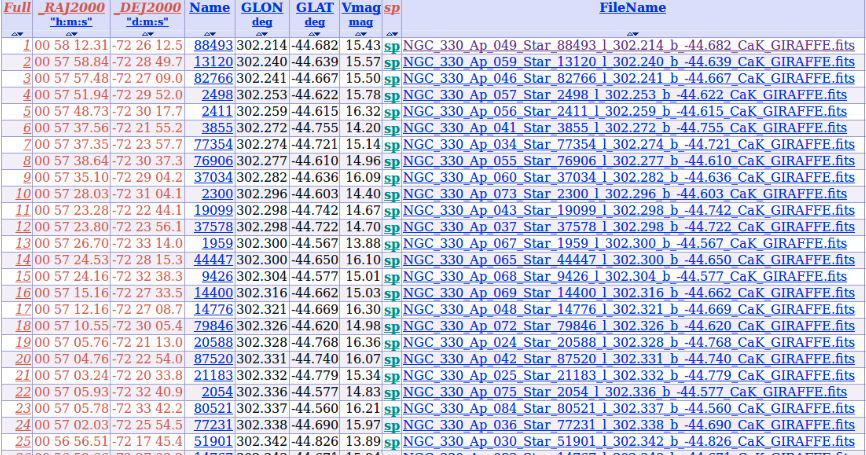
\includegraphics[width=0.9\textwidth]{associated.png}
\caption{catalog of sources with associated time series link}
\label{fig:associated}
\end{figure}



      More information and related Access Data features are detailed in section~\ref{sec:source}.
   \item{ObsCore driven Discovery}

         In this second mode, we consider having a time series repository somewhere, and ObsCore metadata \citep{2017ivoa.spec.0509L} describing them. See "Nebot et al, 2018" for a  list of additional metadata which could be needed for time series Discovery.

          More information and related Access Data features are detailed in section~\ref{sec:obscore}.


    \item{Mixed ObsCore and source physical parameters search}

         In this mode we combine Discovery criteria of Obscore-style with physical parameters describing the time series or the source or astronomical object which has been observed to produce the time series.

More information and related Access Data features are detailed in section~\ref{sec:mixed}.
      \item{Time selection in source catalogues}
      
            Some IVOA protocols (SimpleConeSearch, TMOC) allow to select list of related measurements including TimeStamps. Such list cannot always be considered as TimeSeries. More information is detailed in section~\ref{sec:conesearch}
\end{itemize} 

\section{Source driven Discovery}
\label{sec:source}
       In this case the selection of sources is done through Position (SCS) or through constraints on the column of the catalogue (measurements of  various quantities  or flags associated to the object. These measurements can be generic parameters describing the time series or time-agnostic parameters). At the catalogue level, a selection criterium can be associated on the existence of attached time series as associated dataset to the sources. 


        The response of such a query is a table where each line is a source owning an associated time series.
This can be made available via a URL link associated to each relevant line of the list of sources representation (for example each row of the VOTable TABLE element) 


       The URL allowing to retrieve this time series can be directly given in one of the columns of the response table. In that case and for a VOTable serialisation a LINK element included in this FIELD will contain "application/x-votable+xml;content=timeseries" in its content-type attribute (see figure~\ref{fig:Link}).

\begin{figure}
\centering

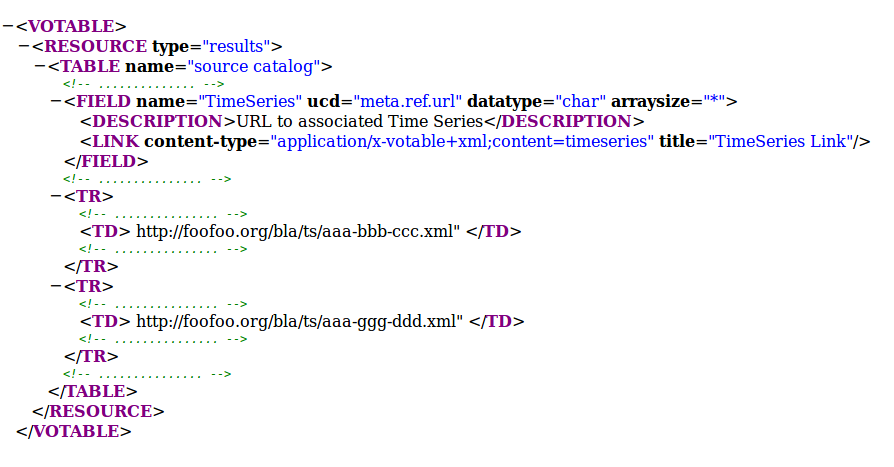
\includegraphics[width=0.9\textwidth]{Link.png}
\caption{LINK element providing content and title information for a URL FIELD}
\label{fig:Link}
\end{figure}


        If the URL is built from a baseURL using one of the table columns  as a "source identifier" this can be done by using a DataLink service descriptor \citep{2015ivoa.spec.0617D} defining the base URL as the root URL of a customized "time series retrieval" service (see figure~\ref{fig:ServiceDescriptor}).

\begin{figure}
\centering

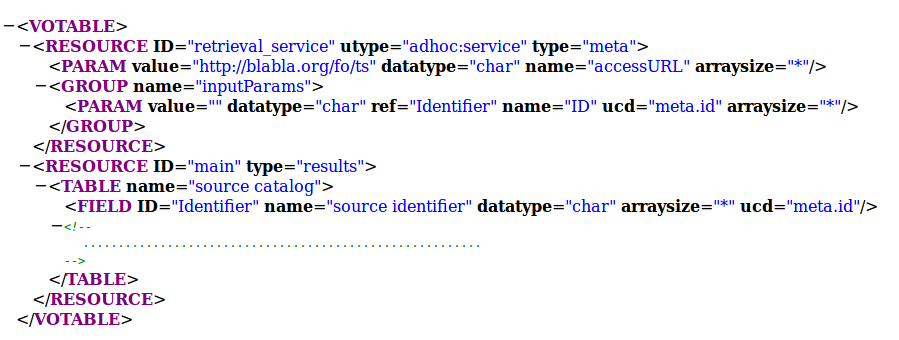
\includegraphics[width=0.9\textwidth]{ServiceDescriptor.png}
\caption{TimeSeries retrieval service descriptor}
\label{fig:ServiceDescriptor}
\end{figure}



        In both cases the client should be able to call the TimeSeries and display it in an appropriate way.

        A variant will propose an access to a  DataLink \{links\} service \citep{2015ivoa.spec.0617D} instead of direct access to the time series. This would allow to propose various plots or SODA-like Access services in addition to the full retrieval link. Semantics, description, the new "content\_qualifier  and format  FIELDs in the \{links\} response will help the user to figure out which is the timeseries retrieval link, and which are additional services, metadata or formats. 

\section{ObsCore (with or without extension) driven discovery}
\label{sec:obscore}

        Time series are Observation DataSets which may be discovered via ObsTAP services. It is possible to restrict queries to time series by forcing a "dataproduct\_type=TimeSeries" constraint.

	Many data providers delivering Time Series consider that ObsCore attributes are sufficient to discover their products.

	However the time series "DataModelling" effort identified specific additional time and observable attributes necessary for a more detailed description of the time series. These new attributes include (not exhaustively) the min and max exposure time per sample and the min and max time span separating samples as well as description of the time frame of the {\bf data} (Nebot et al, 2018). 
        Such an ObsCoreTimeSeriesExtension table could be added by providers in the ivoa schema and combined with ObsCore if needed for "fine-grain" Discovery of the time series.  
        Availability of such an extension of ObsCore in the service should be advertized by the registry.
        
        Beside TAP queries, in the case of images, discovery can be performed by the SIA2 \citep{2015ivoa.spec.1223D} parameter based query interface. DAL WG and SIA authors are now considering to extend the parameter based interface to any kind of dataproducts, by allowing DPTYPE parameter values different from image and cube.
         DPTYPE=timeseries would serve to discover TimeSeries with this interface. 
       In addition we could  add a few optional parameters to SIAP2 to tackle the time axis fine characterisation and the observable axis fine characterisation as stated in the ObsCoreTimeSeriesExtension.  
    

%         The ObsCore table extended in this way could be called TsCore. A TAP service delivering TsCore will be an extension of ObsTAP called TsTAP.
         
        % In the same way that Obscore information can be delivered via the SIAP-2 parameter interface \citep{2015ivoa.spec.1223D}, TsCore information could be searched via an extension of SIAP-2 called "TsSAP" for TimeSeries Simple Access Protocol.
       % The TsSAP extension will add a few parameters to SIAP-2 to tackle the time axis fine characterisation and the observable axis fine characterisation.  

        The access\_reference URL can be an URL to the time series itself or to a DataLink \{links\} response. The latter will allow the linking of various resources beside the full retrieval link (as described in section~\ref{sec:source}).

  

\section{Mixed search case}
\label{sec:mixed}

TimeSeries may be sometimes discribed by the ObsCore(+-TimeSeriesExtension) metadata alongside some other fine-grained, project specific requirements useful to refine the description. This is the case, e.g., of the GAPS (Global Architecture of Planetary Systems) project timeseries, where the ObsCore(+-Extension) metadata are augmented by the host stellar system's details.
In a TAP context, we can imagine solving this by a service delivering both the ObsCore(+-Extension) to describe the time series and additional tables to contain the host system metadata, i.e. simple or flat views of a possible underlying data model.
ObsCore and the model views could share a column (e.g. the obs\_publisher\_did or the obs\_id) as the reference identifier to drive the joins in the search (ADQL) query.
As in the previous case, the access\_reference URL can be a URL to the time series itself or to a DataLink {links} response.
\section{Time selection in source catalogues}
\label{sec:conesearch}
ConeSearch 1.1 allows to select astronomical measurements belonging to specific Time ranges. The result of such queries may be very heterogeneous depending on the nature of the queried catalog. It is  the responsability of the user with the help of appropriate client to organize the ouput in one or several TimeSeries (or not), depending of her scientific goals. A more peculiar and simple case occurs when the catalogue gathers measurements at several times for  different sources.
On line DataBases able to interpret TMOCS (which is both a hierarchical representation of TimeCoverage and an indexation mechanism) may provide the same kind of results.    

\section{Data Access}
\label{sec:access}

      Users may want to access  the whole time series. In that case a "full retrieval" link in the Discovery response is sufficient. In some cases time series may be too huge or too complex to be fully retrieved. Users need a service selecting data extracted from  the time series. Sometimes values could also be transformed to fit user's requests.
Examples of such Access options are:

\begin{itemize}
     \item selection of data points in a Time range
     \item selection of one single scalar observable when several are available (eg select one photometric band in a "multi-band" time series)
     \item selection of a single TARGET  when the TimeSeries gathers several of them.
\end{itemize}
SODA-1.0 interface \citep{2017ivoa.spec.0517B}  allows to provide a lot of selection options similar to those. 
In addition more complex features would be useful, such as :
 \begin{itemize}
      \item extracting a light curve from a cube with a time axis.
      \item conversion of Time Stamps into another Time Scale
      \item rebinning of data on the TimeAxis
      \item merging of data points coming from several catalogs to create a "compilation" time series
\end{itemize}      

 However, currently the output of SODA will be a cube (ie an array of values) of the same dimensions than the archived data. There is no reduction of dimensionality in current SODA interface. Neither is there any transformation of the dataset values.  
 
    For this reason, SODA-1.1 should allow to restrict output datasets to be  "time series" by constraining the criterium (DPTYPE=TimeSeries), to force the nature of the  Observable and to add a transformation interface.  This requires introduction of new SODA parameters such as TIMERES, TIMESCALE,  etc...


  

\section{Summary of DAL actions}
These are the actions to be driven under the DAL responsability:

\begin{itemize}
\item add the "application/x-votable+xml;content=TimeSeries" option to the content-type attribute in LINK element of VOTable
\item support DM working group efforts to build the extension of ObsCore for TimeSeries  using time series specific attributes by extending ObsTAP services to this extension.
\item extend the scope and input parameters of SIAV2 to tackle TimeSeries dataproduct\_type and TimeSeries extension attributes. This may be part of an upgrade of SIAV2 towards a SimpleDataSetAccess protocol.
\item extend SODA input parameters for integrating more acces functionalities. This can be covered by SODA-1.1 including  an optional specialisation for TimeSeries 
\item support the work of adding the TIME parameter in ConeSearch and the recommendation of the TMOC specification.

\end{itemize}
 By the way, support the addition of an STMOC parameter in all the revisions of the simple Access protocols would be a great help.
  
 

The new features proposed here as well as best practices  can be specified in one single   Endorsed Note called "DAL Protocols extensions for Time Series": DALTsExt. These new features as described in this specification document will be added later in the next versions of DAL protocols.   

\appendix

\section{Changes from Previous Versions}
\subsection{Revision1.0-2021-04-30}
\begin{itemize}
\item Adding more authors
\item add a 4th discovery and access mode (Time selection in a catalogue)
\item suppress any special protocol name and replace by extension and optional feature for TimeSeries
\item modify access mode by differentiating selection actions from transformation actions
\item mention STMOC 
\end{itemize}
\subsection{Creation-1.0-2018-07-22}

This is the initial document version. 

\bibliography{ivoatex/docrepo}

\end{document}


